\documentclass[UTF8,zhmap=true,fontset=none,zihao=-4,heading=false,scheme=chinese]{ctexart}
\ctexset{
    punct=kaiming,
    space=auto,
    autoindent=true,
    today=small
}
\setCJKmainfont[BoldFont=SourceHanSerifCN-Heavy, ItalicFont=KaiTi]{SourceHanSerifCN-Regular}% 设置正文罗马族的 CJK 字体,影响 \rmfamily 和 \textrm 的字体。
\setCJKsansfont{SourceHanSansCN-Regular}% 设置正文无衬线族的 CJK 字体,影响 \sffamily 和 \textsf 的字体。
\setCJKmonofont{FangSong}% 设置正文等宽族的 CJK 字体,影响 \ttfamily 和 \texttt 的字体。

\usepackage{hyperref}
\hypersetup{
    colorlinks=true,
    linkcolor=blue,
    filecolor=magenta,      
    urlcolor=cyan,
}

\usepackage{graphicx}
\graphicspath{{figures/}}
\usepackage{subfigure}
\usepackage{caption}

\usepackage{verbatim}

\title{子课题五``水下声呐-视觉SLAM''开发环境配置教程}
\author{肖书奇}
\date{\today}
\begin{document}
\maketitle
\section{简述}
\par 为方便陆老师及课题组其他同学开展后续研究,整理此文档。目前,本文主要内容包括SVIn2与声纳仿真器的开发环境配置与使用方法。
\par 本人已将SVIn2与声纳仿真器分别封装为两个Docker\href{https://docs.docker.com/}{(官方文档)} 镜像,上传至\href{https://hub.docker.com/u/xiaosq2000}{docker hub},
对应的Dockerfile与示例脚本上传至\href{https://github.com/xiaosq2000/SVI-SLAM}{Github}。
\par 这里介绍在Windows系统中利用WSL\href{https://docs.microsoft.com/en-us/windows/wsl/}{(官方文档)} 虚拟机使用Docker,并且通过X server\href{https://en.wikipedia.org/wiki/X_Window_System}{(维基百科)}获取可视化界面的方法。
\par 您当然可以直接在Linux系统中运行Docker\footnote{由于本人的笔记本电脑性能与储存空间极为有限,不具备使用Linux双系统或者完整的虚拟机的条件,才不得已使用WSL,踩坑无数。},通过X server或者VNC等方法获取可视化界面,但目前本教程不涉及此内容。
\section{WSL2-Docker-VcXsrv环境配置}
\subsection{WSL2}
\begin{enumerate}
    \item 您的系统必须是Windows 10版本2004及更高版本(内部版本19041及更高版本)或Windows 11方可安装WSL2。
    \item 建议您使用Windows 11内部版本22000或更高版本,获得对Linux GUI的完整支持,否则Rviz或Gazebo可能会出现最讨厌的Segmentation Fault错误。
    \item 建议您安装vGPU驱动程序,使您可以在虚拟机中使用硬件加速 OpenGL 渲染。
    \begin{itemize}
        \item \href{https://www.intel.com/content/www/us/en/download/19344/intel-graphics-windows-10-windows-11-dch-drivers.html}{适用于WSL的Intel GPU驱动程序}
        \item \href{https://www.amd.com/en/support/kb/release-notes/rn-rad-win-wsl-support}{适用于WSL的AMD GPU驱动程序}
        \item \href{https://developer.nvidia.com/cuda/wsl}{适用于WSL的NVIDIA GPU驱动程序}
    \end{itemize}
    \item 使用管理员特权打开命令提示符:选择“开始”,键入 \verb|PowerShell|,右键单击``Windows PowerShell'',然后选择``以管理员身份运行''。
    \item 运行 \verb|wsl --install -d Ubuntu|,过程中会提示您重启计算机。
    \item 计算机完成重启后,安装将继续进行,并要求你输入用户名和密码。
\end{enumerate}
\subsection{Docker Desktop}
\begin{enumerate}
    \item \href{https://desktop.docker.com/win/main/amd64/Docker%20Desktop%20Installer.exe?utm_source=docker&utm_medium=webreferral&utm_campaign=dd-smartbutton&utm_location=module}{点击此链接下载Docker Desktop (Windows)并安装}
    \item 打开Docker Desktop的设置,在Resources\(\rightarrow\)WSL INTEGRATION中开启Ubuntu,点击Apply \& Restart。
    \item 打开刚装好的WSL2 Ubuntu虚拟机,输入 \verb|docker -h| 检测docker是否可以正常使用。
\end{enumerate}
\begin{figure}
    \centering
    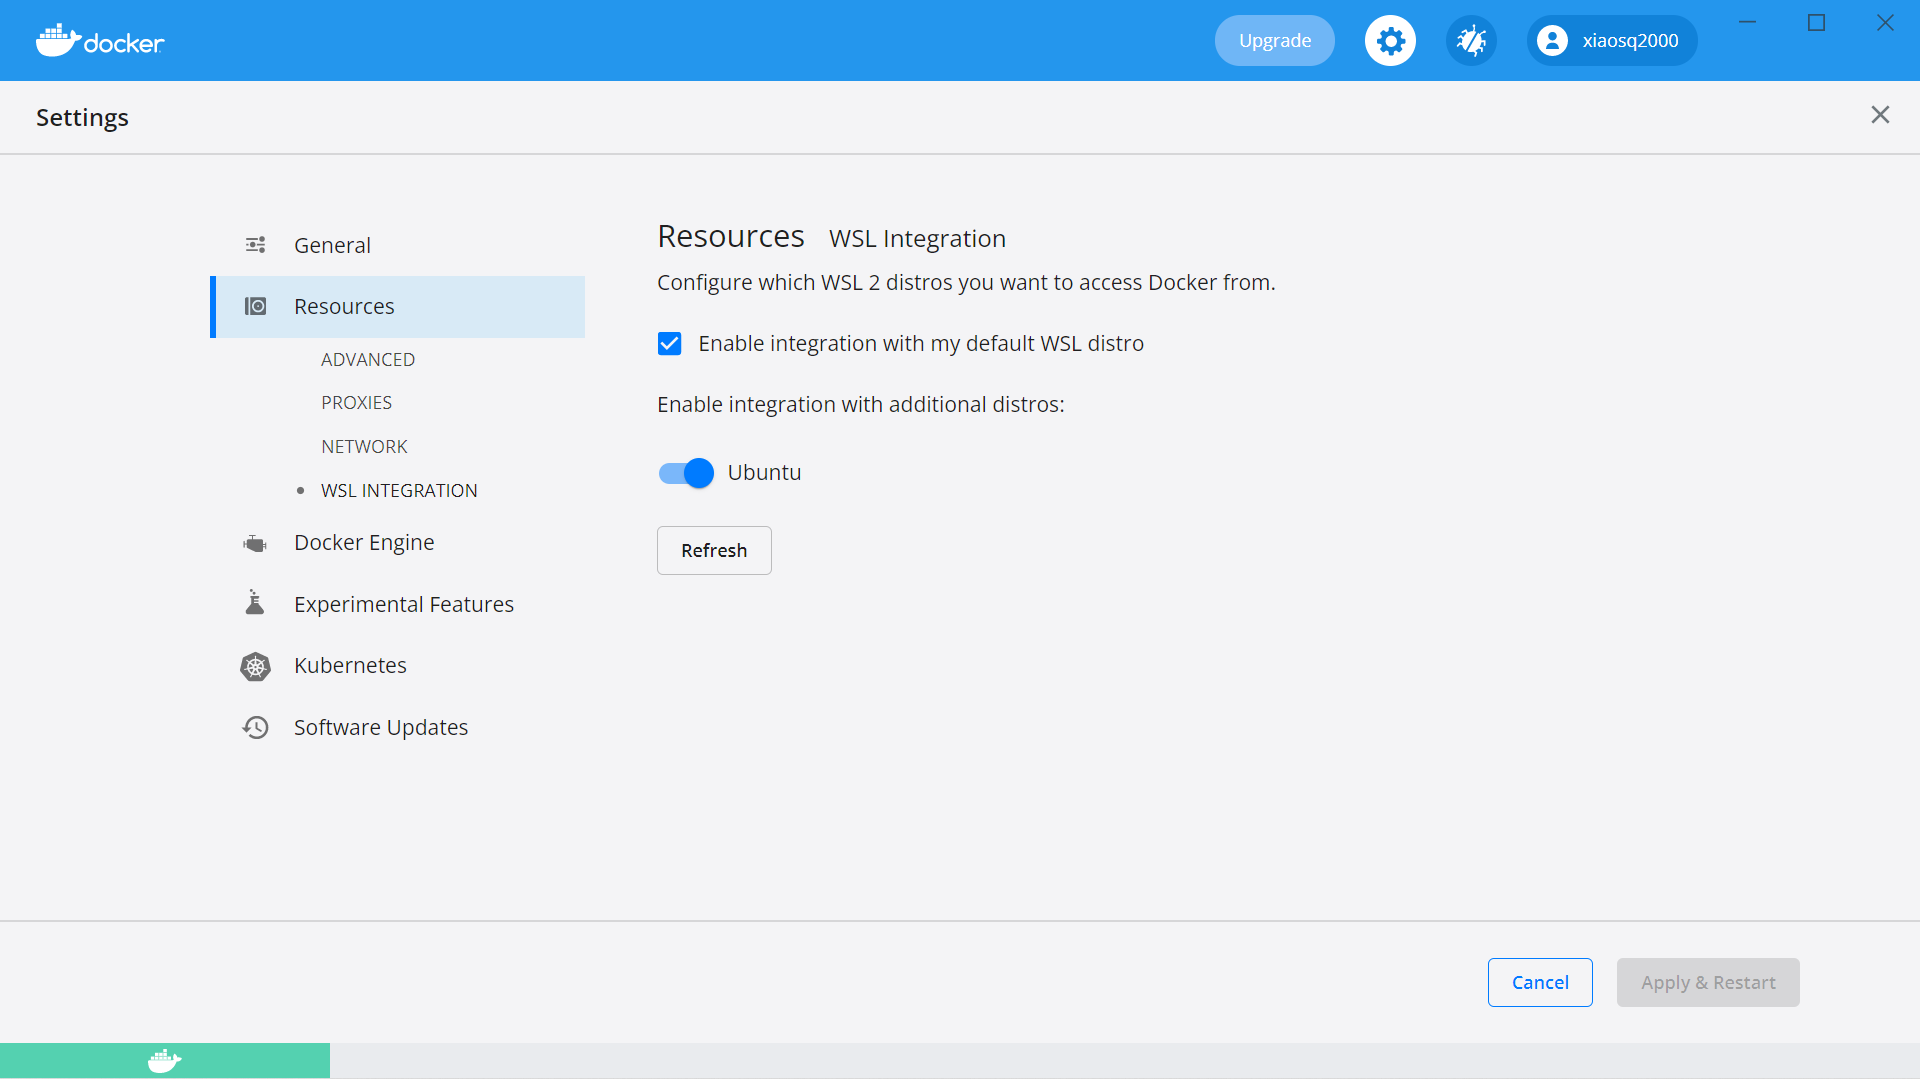
\includegraphics[width=\linewidth]{Docker-Desktop.png}
    \caption{Docker Desktop设置}
\end{figure}
\subsection{VcXsrv Windows X Server}
\begin{enumerate}
    \item \href{https://desktop.docker.com/win/main/amd64/Docker%20Desktop%20Installer.exe?utm_source=docker&utm_medium=webreferral&utm_campaign=dd-smartbutton&utm_location=module}{点击此链接(可能需要VPN)下载VcXsrv Windows X Server并安装}
    \item 打开XLaunch,作出如下设置
\footnote{默认勾选的Native Opengl意味着开启硬件加速渲染,这需要驱动支持,还需要在X client中设置环境变量LIBGL\_ALWAYS\_INDIRECT=1;若取消勾选此项则使用软件渲染,虽然速度更慢,但不易报错,建议您初次使用取消Native OpenGL功能。}
\footnote{可以点击Save configuration,以后打开X server无需重复配置,双击即可。}
\end{enumerate}
\begin{figure}
    \centering
    \subfigure[保持默认选项]{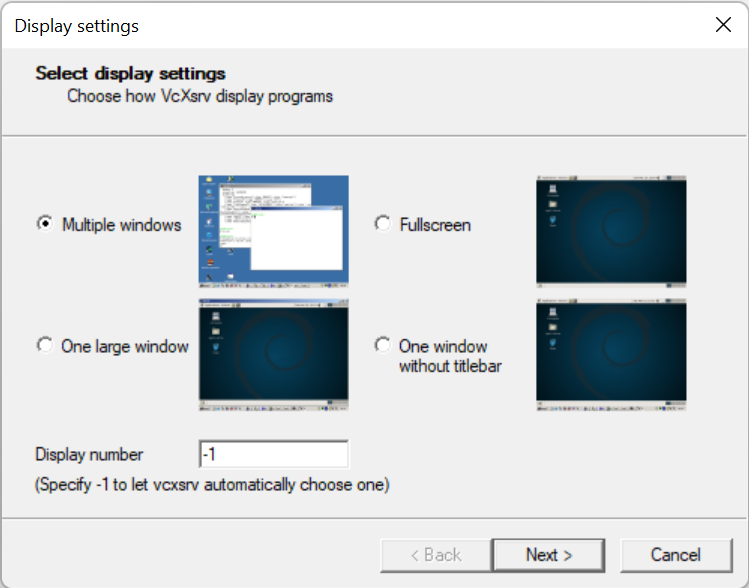
\includegraphics[width=0.45\linewidth]{XLaunch-config-1.png}}
    \quad 
    \subfigure[保持默认选项]{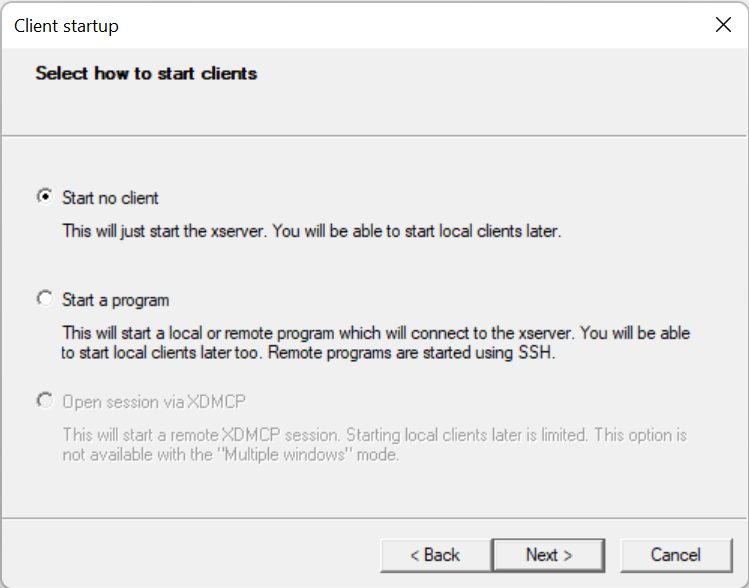
\includegraphics[width=0.45\linewidth]{XLaunch-config-2.png}}
    \\
    \subfigure[务必勾选Disable access control]{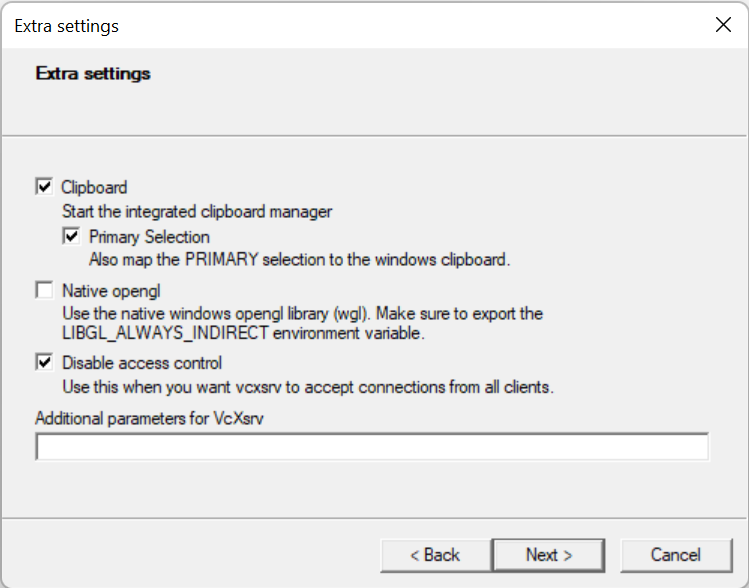
\includegraphics[width=0.45\linewidth]{XLaunch-config-3.png}}
    \quad 
    \subfigure[点击Finish]{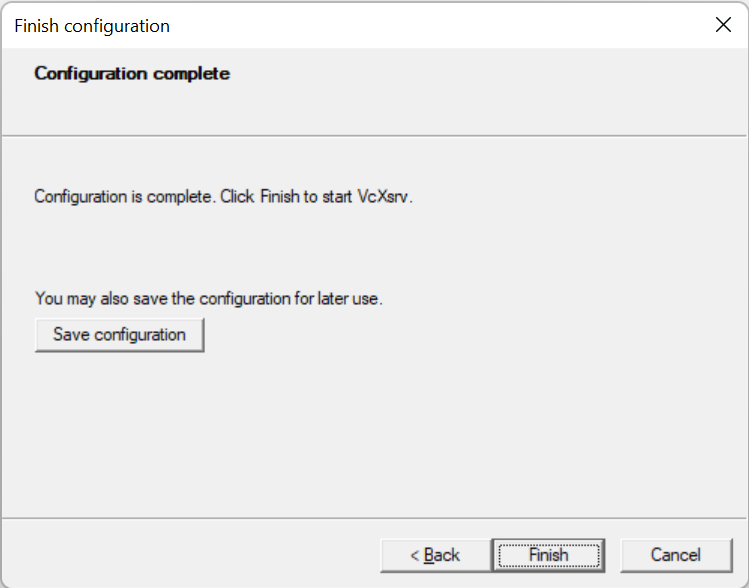
\includegraphics[width=0.45\linewidth]{XLaunch-config-4.png}}
    \caption{XLaunch配置}
\end{figure}
\par 至此,您的WSL2-Docker-VcXsrv环境准备完毕。
\section{svin2与sonar\_simulation环境}
\begin{enumerate}
    \item 打开两个WSL2 Ubuntu终端,分别输入 \\
    \verb|docker pull xiaosq2000/svin2:latest| \\ 
    \verb|docker pull xiaosq2000/sonar_simulation:latest| \\ 
    同时拉取两个Docker镜像,总共约10GB。下载完毕后,可以在Docker Desktop中看到这两个镜像。
    \item 打开WSL2 Ubuntu终端,在您认为合适的文件夹中输入 \\
    \verb|git clone https://github.com/xiaosq2000/SVI-SLAM| \\ 
\end{enumerate}
\par 至此,您的Docker镜像与示例脚本准备完毕。
\subsection{svin2}
\begin{enumerate}
    \item 准备好AFRL实验室的rosbag数据集
    \item 编辑\verb|SVI-SLAM/docker_images/svin2/scripts/run_test_container.sh|
    \begin{itemize}
        \item 第6行的含义是以只读模式挂载文件夹到Docker容器中。由于本人的数据集放在Windows系统的\verb|C:/datasets/SVIn2-datasets/|中,所以对应内容为\verb|source=/mnt/c/datasets/SVIn2-datasets|,请替换为您的路径。
        \item 删除第11、12、13、14行。\footnote{如果您不使用网络代理(仅是运行例程无需网络)}
        \item 删除第17行。\footnote{如果您不使用vim}
    \end{itemize}
    \item 删除\verb|SVI-SLAM/docker_images/svin2/scripts/personal_config.sh|的第2、3行,或替换为您的个人信息。
    \item 运行 \verb|run_test_container.sh| 即可。
    \item 键盘输入\verb|Ctrl+C|即可退出仿真,在Docker容器中进行其他操作。
    \item 输入\verb|exit|即可退出Docker容器,回到WSL2 Ubuntu终端。
\end{enumerate}
\subsection{sonar\_simulation}
\begin{enumerate}
    \item 删除\\\verb|SVI-SLAM/docker_images/sonar_simulation/scripts/run_test_container.sh|\\的第10、11、12、13、16行。
    \item 运行 \verb|run_test_container.sh| 即可。
    \item 键盘输入\verb|Ctrl+C|即可退出仿真,在Docker容器中进行其他操作。
    \item 输入\verb|exit|即可退出Docker容器,回到WSL2 Ubuntu终端。
\end{enumerate}

\end{document}
